\documentclass[11pt]{article}
\usepackage[utf8]{inputenc}
\usepackage[T1]{fontenc}
\usepackage{geometry}
\usepackage{hyperref}
\usepackage{enumitem}
\usepackage{tikz}
\usetikzlibrary{positioning}

\geometry{margin=1in}

\title{BS Portfolio 01 MealPlanner}
\author{
  \textit{[Author Name 1]} (\textit{[Matriculation Number]})\\
  \textit{[Author Name 2]} (\textit{[Matriculation Number]})
}
\date{October 27, 2025}

\begin{document}

\maketitle

\section{Project Overview}

\textbf{The Problem.} Food prices for similar products vary dramatically – often by several multiples. Even when comparing different foods based on their nutritional value (proteins, carbohydrates, fats), there are huge price differences per unit of nutrition. This makes it difficult for consumers to make informed decisions about which foods best fit their goals and budget.

\textbf{Our Solution.} The MealPlanner backend allows users to register food items with their prices and nutritional values (e.g., "Barilla Lasagne Sheets n.189" with specific nutritional data). The system can then filter and sort these foods by various criteria such as:
\begin{itemize}[noitemsep]
  \item Price per 100g protein
  \item Price per 1000 calories
  \item Protein content per 100g
  \item And many other nutritional and cost metrics
\end{itemize}

This helps users make better decisions about which foods fit their personal goals while achieving them cost-effectively.

\textbf{Dish Management.} Users can also create dishes by adding multiple DishIngredients (ideally as lists) and filter them using the same criteria – total protein, total carbs, etc. – just like individual food items. This allows users to achieve their goals in a budget-friendly and macro-compliant way. Dishes can include preparation descriptions and time requirements, with filtering options by preparation time.

\textbf{Technical Implementation.} The MVP delivers CRUD management for \texttt{FoodItem} and \texttt{Dish} resources. 

\textbf{Scope Limitations.} The first increment explicitly excludes allergen/micronutrient modeling, user accounts, and automated meal-plan generation to keep the deliverable focused.

\section{Domain Model}

The core entities and relationships appear in Figure~\ref{fig:uml}. The domain layer ensures each dish retains at least one ingredient line, and every line records the gram quantity that drives deterministic cost and macronutrient calculations.

\begin{figure}[h]
  \centering
  \resizebox{0.9\linewidth}{!}{%
  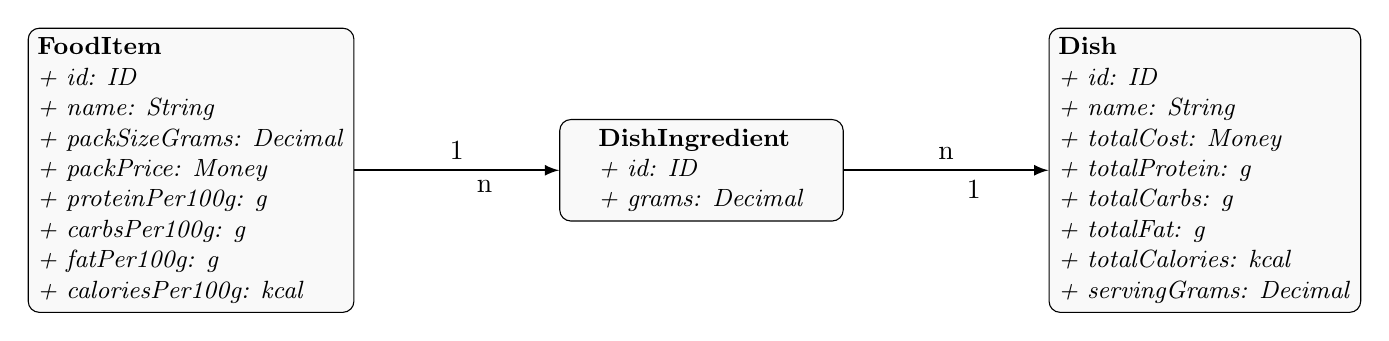
\begin{tikzpicture}[
    class/.style={rectangle, draw, rounded corners, minimum width=3.6cm, align=left, font=\small, fill=gray!5},
    relation/.style={-latex, thick},
    node distance=2.6cm
  ]

    \node[class] (food) {
      \textbf{FoodItem}\\
      \textit{+ id: ID}\\
      \textit{+ name: String}\\
      \textit{+ packSizeGrams: Decimal}\\
      \textit{+ packPrice: Money}\\
      \textit{+ proteinPer100g: g}\\
      \textit{+ carbsPer100g: g}\\
      \textit{+ fatPer100g: g}\\
      \textit{+ caloriesPer100g: kcal}
    };

    \node[class, right=of food] (dishIng) {
      \textbf{DishIngredient}\\
      \textit{+ id: ID}\\
      \textit{+ grams: Decimal}
    };

    \node[class, right=of dishIng] (dish) {
      \textbf{Dish}\\
      \textit{+ id: ID}\\
      \textit{+ name: String}\\
      \textit{+ totalCost: Money}\\
      \textit{+ totalProtein: g}\\
      \textit{+ totalCarbs: g}\\
      \textit{+ totalFat: g}\\
      \textit{+ totalCalories: kcal}\\
      \textit{+ servingGrams: Decimal}
    };

    \draw[relation] (food) -- node[above]{1} node[below]{\quad\quad n} (dishIng);
    \draw[relation] (dishIng) -- node[above]{n} node[below]{\quad\quad 1} (dish);
  \end{tikzpicture}%
  }
  \caption{UML class diagram of the Meal Planner domain.}
  \label{fig:uml}
\end{figure}

\paragraph{Key entities.} \textbf{FoodItem} stores its pack size and price alongside nutritional facts per 100\,g, allowing the service to derive cost metrics such as price per 100\,g. \textbf{DishIngredient} records only the grams of a referenced food item; all macro shares are derived on demand. \textbf{Dish} aggregates ingredients and persists the latest totals (cost, protein, carbohydrates, fat, calories) together with \textit{servingGrams} so ranking endpoints can query efficiently without recomputing every aggregation on read.

\paragraph{Domain invariants.}
\begin{itemize}[noitemsep]
  \item Pack price and size must be positive; macro values per 100\,g remain within plausible physiological limits.
  \item DishIngredient entries require strictly positive grams; operations that leave a dish empty are rejected.
  \item Aggregated dish totals (cost and macronutrients) are recalculated transactionally in the domain layer by multiplying each \texttt{FoodItem} profile with its recorded grams, rounded to two decimals, and persisted together with \texttt{servingGrams} to support fast sorting and paging.
\end{itemize}

\paragraph{Example records.}
\begin{itemize}[noitemsep]
  \item FoodItem: \emph{``Chicken Breast''}, pack size 1{,}000\,g, pack price 7{,}50\,€, protein 23\,g/100\,g, carbohydrates 0\,g/100\,g, fat 1{,}5\,g/100\,g, calories 110\,kcal/100\,g.
  \item Dish: \emph{``Budget Protein Bowl''} with 150\,g Chicken Breast, 100\,g Rice, and 50\,g Broccoli, yielding a total cost of 2{,}45\,€, 38\,g protein, 58\,g carbohydrates, 11\,g fat, and 510\,kcal.
\end{itemize}

\section{Use Cases}

The backend covers four core use cases. Each outlines priority, preconditions, main steps, alternate flows, postconditions, and acceptance criteria.

\subsection*{UC01 -- Register Food Item (Must)}
\textbf{Primary Actor:} Data curator.\\
\textbf{Goal (User Story):} ``As a curator, I want to register a base ingredient with reliable macro values and pricing so dishes can use authoritative data.''\\
\textbf{Preconditions:} Ingredient name is unique; macro and price fields are present and valid.\\
\textbf{Main Success Scenario:}
\begin{enumerate}[label=\arabic*.]
  \item The actor submits \texttt{POST /food-items} with name, macros per 100\,g, unit price, and timestamps.
  \item The domain validates ranges, then persists the \texttt{FoodItem} via the persistence port.
  \item The API returns \texttt{201 Created} with the identifier and echo data.
\end{enumerate}
\textbf{Alternate / Failure Flows:}
\begin{enumerate}[label=\arabic*F.]
  \item Duplicate name $\rightarrow$ \texttt{409 Conflict} with guidance to adjust the identifier.
  \item Validation error (e.g., negative macros) $\rightarrow$ \texttt{400 Bad Request} with constraint details.
\end{enumerate}
\textbf{Postconditions:} FoodItem stored and available for dish composition.\\
\textbf{Acceptance Criteria:}
\begin{itemize}[noitemsep]
  \item Numeric inputs persist with two-decimal precision; negatives are rejected.
  \item Unit tests cover validation boundaries and duplicate handling.
\end{itemize}

\subsection*{UC02 -- Compose Dish (Must)}
\textbf{Primary Actor:} Nutrition planner.\\
\textbf{Goal (User Story):} ``As a planner, I want to assemble a dish from precise ingredient weights so MealPlanner calculates totals automatically.''\\
\textbf{Preconditions:} At least one \texttt{FoodItem} exists; gram weights are positive.\\
\textbf{Main Success Scenario:}
\begin{enumerate}[label=\arabic*.]
  \item The actor calls \texttt{POST /dishes} with name, servings, and an ingredient list (\texttt{foodItemId}, grams).
  \item The application service loads referenced ingredients and recomputes totals and ranking metrics.
  \item The transaction persists the \texttt{Dish} and \texttt{DishIngredient} entities atomically.
  \item The API returns \texttt{201 Created} with calculated totals and optimistic-lock metadata.
\end{enumerate}
\textbf{Alternate / Failure Flows:}
\begin{enumerate}[label=\arabic*F.]
  \item Unknown \texttt{foodItemId} $\rightarrow$ \texttt{404 Not Found}.
  \item Ingredient grams $\leq 0$ $\rightarrow$ \texttt{400 Bad Request} with validation hints.
\end{enumerate}
\textbf{Postconditions:} Dish totals reflect submitted ingredients.\\
\textbf{Acceptance Criteria:}
\begin{itemize}[noitemsep]
  \item Calculated totals equal the sum of ingredient contributions within rounding tolerance.
  \item Integration tests confirm persistence and retrieval reproduce totals verbatim.
\end{itemize}

\subsection*{UC03 -- Adjust Dish Composition (Should)}
\textbf{Primary Actor:} Nutrition planner.\\
\textbf{Goal (User Story):} ``As a planner, I want to adjust ingredient weights so cost-per-protein metrics remain trustworthy over time.''\\
\textbf{Preconditions:} The target dish exists and references at least one ingredient.\\
\textbf{Main Success Scenario:}
\begin{enumerate}[label=\arabic*.]
  \item The actor modifies the composition using sub-resources:
    \begin{itemize}[noitemsep]
      \item Add: \texttt{POST /dishes/\{dishId\}/ingredients} with \{\texttt{foodItemId}, \texttt{grams}\}.
      \item Update: \texttt{PATCH /dishes/\{dishId\}/ingredients/\{dishIngredientId\}} with \{\texttt{grams}\}.
      \item Remove: \texttt{DELETE /dishes/\{dishId\}/ingredients/\{dishIngredientId\}}.
    \end{itemize}
  \item The domain reapplies validation and recomputes totals, ratios, and derived rankings.
  \item The persistence layer applies changes in a transaction and updates audit timestamps.
  \item The API returns the refreshed \texttt{Dish} representation with version metadata.
\end{enumerate}
\textbf{Alternate / Failure Flows:}
\begin{enumerate}[label=\arabic*F.]
  \item Dish locked by another transaction $\rightarrow$ \texttt{409 Conflict} with retry advice.
  \item Removing all ingredients $\rightarrow$ \texttt{400 Bad Request}, message ``Dish must contain at least one ingredient.''
\end{enumerate}
\textbf{Postconditions:} Dish reflects new macro and cost totals.\\
\textbf{Acceptance Criteria:}
\begin{itemize}[noitemsep]
  \item Integration tests ensure per-serving calculations refresh after modifications.
  \item Optimistic locking prevents concurrent overwrites without warning.
\end{itemize}

\subsection*{UC04 -- Retrieve Ranked Dishes (Must)}
\textbf{Primary Actor:} Shopper preparing meal plans.\\
\textbf{Goal (User Story):} ``As a shopper, I want to list dishes sorted by specific value metrics so I can select the most cost-effective meals quickly.''\\
\textbf{Preconditions:} At least one dish with aggregated metrics exists; pagination defaults are configured.\\
\textbf{Main Success Scenario:}
\begin{enumerate}[label=\arabic*.]
  \item The actor calls \texttt{GET /dishes} with query parameters for sorting, filtering, and paging, e.g.:\\
  \texttt{/dishes?sort=pricePerProtein:asc,name:asc\&page=0\&size=20\&minProtein=30}
  \item The application service issues a database query with the corresponding \texttt{ORDER BY} clause and pagination window.
  \item The API returns a paginated JSON list with rank numbers, summary metrics, and hypermedia links (\texttt{Link} headers or body) to adjacent pages.
\end{enumerate}
\textbf{Alternate / Failure Flows:}
\begin{enumerate}[label=\arabic*F.]
  \item No dishes found $\rightarrow$ \texttt{200 OK} with empty array.
  \item Unsupported sort field $\rightarrow$ \texttt{400 Bad Request} listing valid options.
\end{enumerate}
\textbf{Postconditions:} User receives ordered dish list for immediate comparison.\\
\textbf{Acceptance Criteria:}
\begin{itemize}[noitemsep]
  \item Sorting stays stable via deterministic tie-breakers (e.g., \texttt{name}, then \texttt{id}).
  \item Integration tests assert ordering, filters, pagination metadata, caching headers, and hypermedia navigation.
\end{itemize}

\end{document}
